\documentclass{article}

\usepackage{graphicx}
\usepackage{tikz}
\usepackage{tikzsymbols}
\usetikzlibrary{calc,patterns,shapes.geometric}
\pagestyle{empty}
\usepackage[margin=0pt]{geometry}
\geometry{papersize={14in,12in}}

\def\centerarc[#1](#2)(#3:#4:#5){\draw[#1] ($(#2)+({#5*cos(#3)},{#5*sin(#3)})$) arc (#3:#4:#5);}

\begin{document}
	\begin{figure}
		\centering
		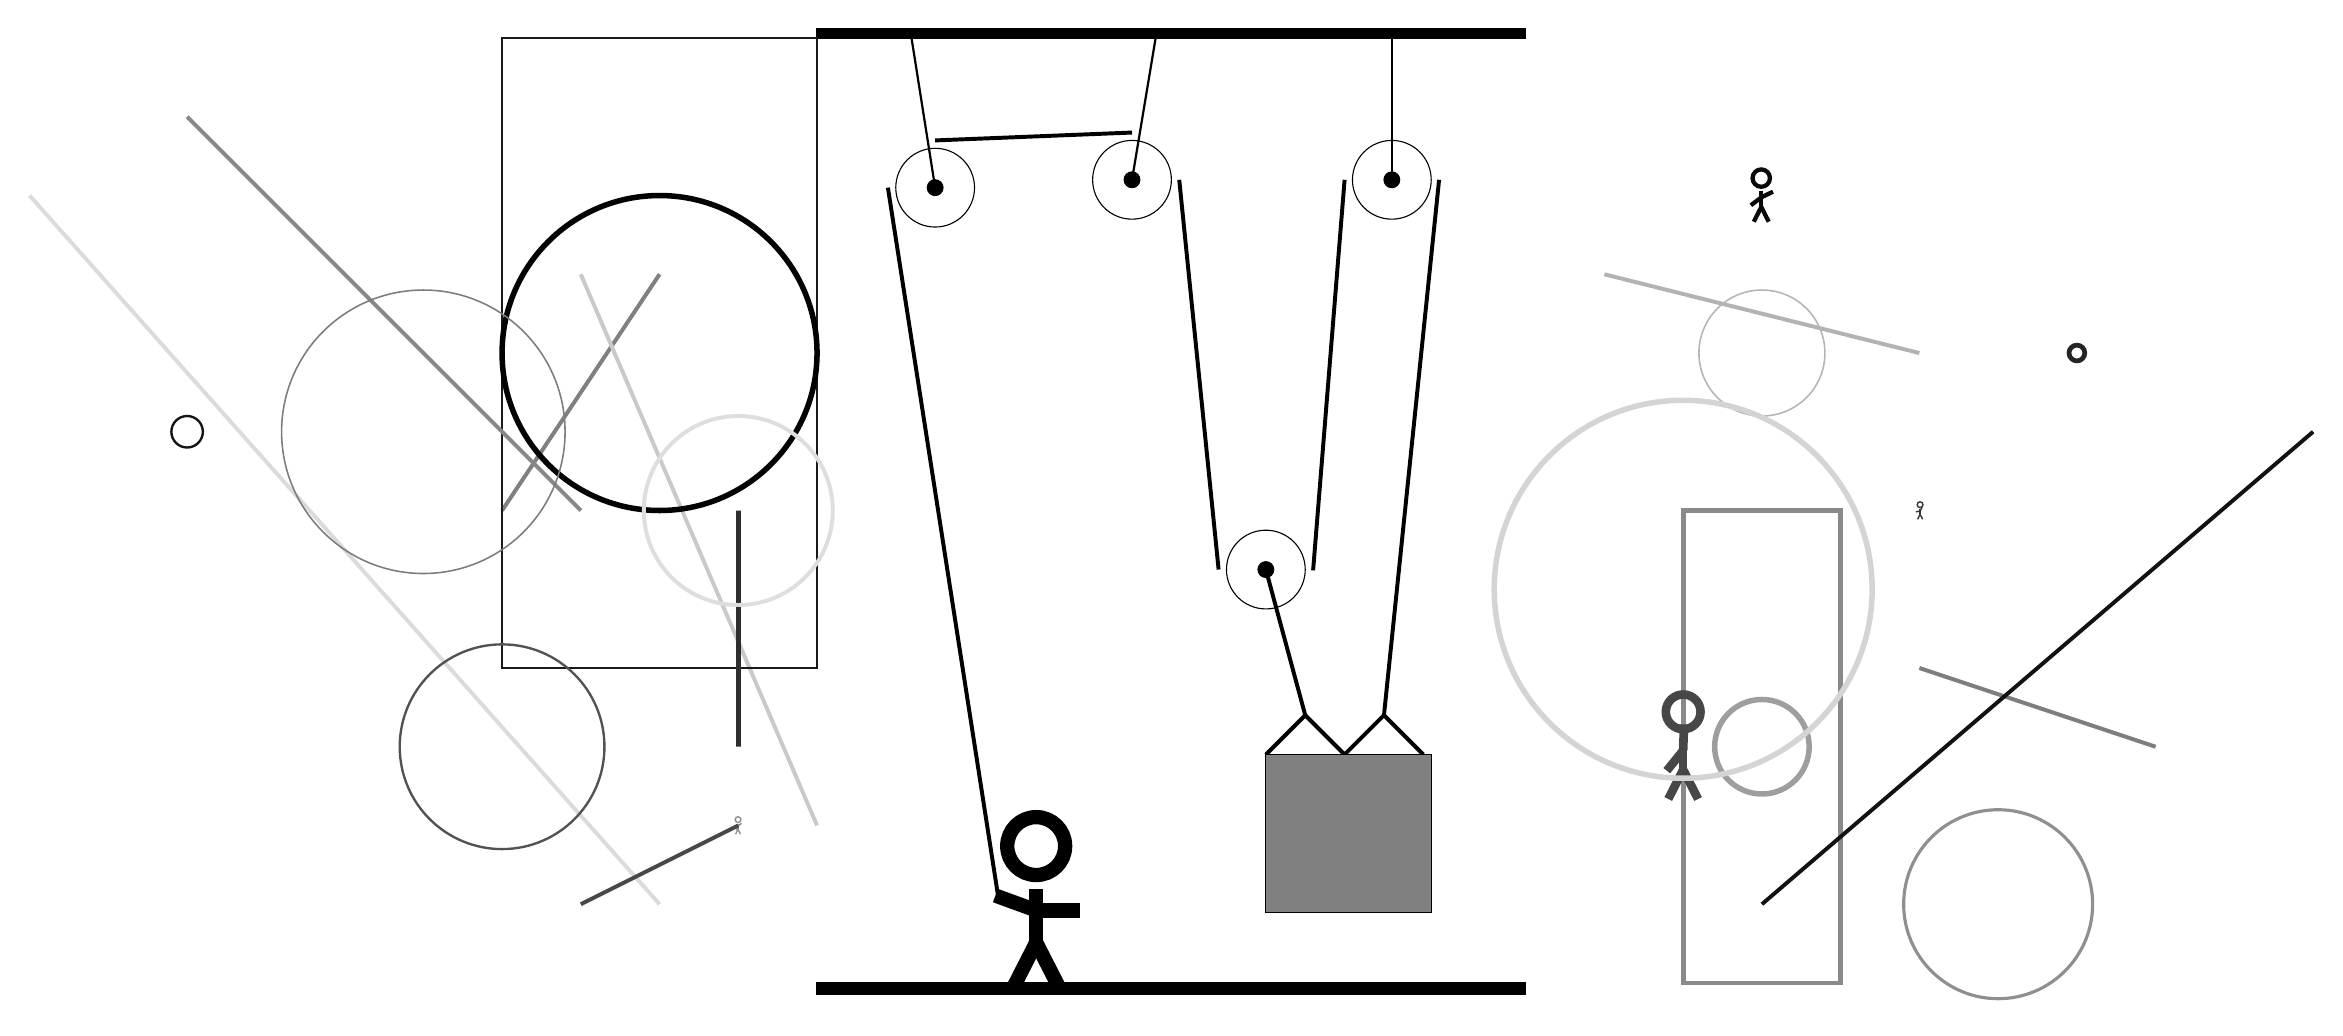
\begin{tikzpicture}
			%%%%% START %%%%%
			
			\draw[fill=black] (-3, 9) rectangle (6, 9.125);
			
			\draw (1, 7.2) circle (0.5);
			\draw[fill=black] (1, 7.2) circle (0.1);
			\draw[thick] (1, 7.2) -- (1.3, 9);
			
			\node[line width=0.5mm, color=black!43] at (-4, -1) {\Strichmaxerl[1][71][39]};
			
			\draw[line width=0.5mm, color=black!50](-7, 3) -- (-5, 6);
			\draw[line width=0.5mm, color=black!21](-6, 6) -- (-3, -1);
			\draw[line width=0.6mm, color=black!46] (8, -3) rectangle (10, 3);
			\draw[line width=0.5mm, color=black!14](-5, -2) -- (-13, 7);
			\node[line width=0.5mm, color=black!72] at (8, 0) {\Strichmaxerl[6][51][88]};
			
			\draw[line width=0.3mm, color=black!90] (-3, 1) rectangle (-7, 9);
			\draw[line width=0.5mm, color=black!72](-6, -2) -- (-4, -1);
			\draw[line width=0.5mm, color=black!51](11, 1) -- (14, 0);
			
			\draw [line width=0.4mm, color=black!44](12, -2) circle (1.2);
			
			\draw [line width=0.7mm, color=black!99](-5, 5) circle (2.0);
			\draw[line width=0.5mm, color=black!93](9, -2) -- (16, 4);
			\draw[line width=0.6mm, color=black!82] (-4, 3) rectangle (-4, 0);
			
			\draw [line width=0.5mm, color=black!13](-4, 3) circle (1.2);
			\draw[line width=0.5mm, color=black!47](-6, 3) -- (-11, 8);
			\draw[line width=0.5mm, color=black!30](7, 6) -- (11, 5);
			\draw [line width=0.6mm, color=black!86](13, 5) circle (0.1);
			\draw [line width=0.2mm, color=black!51](-8, 4) circle (1.8);
			\node[line width=0.4mm, color=black!96] at (9, 7) {\Strichmaxerl[3][37][26]};
			
			\draw [line width=0.2mm, color=black!29](9, 5) circle (0.8);
			\draw [line width=0.3mm, color=black!68](-7, 0) circle (1.3);
			\node[line width=0.7mm, color=black!79] at (11, 3) {\Strichmaxerl[1][9][63]};
			\draw [line width=0.7mm, color=black!38](9, 0) circle (0.6);
			\draw [line width=0.7mm, color=black!17](8, 2) circle (2.4);
			\draw [line width=0.3mm, color=black!92](-11, 4) circle (0.2);
			
			\draw (4.3, 7.2) circle (0.5);
			\draw[fill=black] (4.3, 7.2) circle (0.1);
			\draw[thick] (4.3, 7.2) -- (4.3, 9);
			
			\draw (2.7, 2.25) circle (0.5);
			\draw[fill=black] (2.7, 2.25) circle (0.1);
			
			\draw[line width=0.5mm]  (2.7, -0.1) -- (3.2, 0.4) -- (3.7, -0.1) -- (4.2, 0.4) -- (4.7, -0.1);
			\draw[fill=black!50] (2.7, -0.1) rectangle (4.8, -2.1);
			
			\draw (-1.5, 7.1) circle (0.5);
			\draw[fill=black] (-1.5, 7.1) circle (0.1);
			\draw[thick] (-1.5, 7.1) -- (-1.8, 9);
			
			\draw[line width=0.5mm](-0.7, -1.9) --  (-2.1, 7.1);
			\centerarc[line width=0.5mm](-1.5, 7.1)(90:180:0.6);
			\draw[line width=0.5mm](-1.5, 7.7) -- (1, 7.8);
			\centerarc[line width=0.5mm](1, 7.2)(0:90:0.6);
			\draw[line width=0.5mm](1.6, 7.2) -- (2.1, 2.25);
			\centerarc[line width=0.5mm](2.7, 2.25)(180:370:0.6);
			\draw[line width=0.5mm] (3.3, 2.24) -- (3.7, 7.2);
			\centerarc[line width=0.5mm](4.3, 7.2)(0:180:0.6);
			\draw[line width=0.5mm](4.2, 0.4) -- (4.9, 7.2);
			\draw[line width=0.5mm] (3.2, 0.4) -- (2.7, 2.25);
			
			\node at (-0.2, -2) {\Strichmaxerl[10][-20][0]};
			
			\draw[fill=black] (-3, -3) rectangle (6, -3.15);
			
			%%%%% END %%%%%
		\end{tikzpicture}
	\end{figure}	
\end{document}